%%%%%%%%%%%%%%%%%%%%%%%%%%%%%%%%%%%%%%%%%%%%%%%%%%%%%%%%%%%%%%%%%%%%%%%%%%%%%%%%%%%%%
% BiuldSim2020_paper_format_guide.tex Revised by: Mandana S. Khanie, masak@byg.dtu.dk
% It is a modification of the master file made by Alessandro Prada, alessandro.prada@unint.it
%%%%%%%%%%%%%%%%%%%%%%%%%%%%%%%%%%%%%%%%%%%%%%%%%%%%%%%%%%%%%%%%%%%%%%%%%%%%%%%%%%%%%

\documentclass[twocolumn, a4paper,10pt]{article}
\usepackage[top=2.5cm, bottom=2.5cm, left=2.0cm, right=2.0cm,
columnsep=0.8cm]{geometry}
\usepackage{enumitem}
\usepackage[hidelinks]{hyperref}
\usepackage{boxedminipage}
\usepackage{nopageno}
\usepackage{graphicx}
\usepackage{natbib}
\usepackage[font=it]{caption}
\usepackage[usenames,dvipsnames]{xcolor}
\usepackage{listings}
\usepackage{caption}
\usepackage{subcaption}
\usepackage{algorithm}
\usepackage{algorithmic}
\newcommand{\pluseq}{\mathrel{+}=}


%-----------------------------SET SKIP SPACES -------------------------------------------------------------------
\setlength{\abovecaptionskip}{0pt}
\setlength{\belowcaptionskip}{3pt}
\setlength{\parindent}{0pt}
\setlength{\parskip}{3pt}
%\renewcommand{\baselinestretch}{0.7}
% FOR enumerates
\setlist{itemsep=-0.1cm,topsep=0.1cm,labelsep=0.3cm}
\setenumerate{leftmargin=*}
\setcounter{secnumdepth}{-1}
%-----------------------------SET FONTS -------------------------------------------------------------------
% Set fonts for title, section and subsection headings
\makeatletter
\renewcommand\title[1]{\gdef\@title{\fontsize{12pt}{2pt}\bfseries{#1}}}
\makeatletter
\renewcommand\section{\@startsection{section}{1}{\z@}{3pt}{3pt}{\normalfont\large\bfseries}}
% \normalfont\large
\makeatletter
\renewcommand\subsection{\@startsection{subsection}{1}{\z@}{\z@}{\z@}{\normalfont\normalsize\bfseries}}
\makeatletter
\renewcommand\subsection{\@startsection{subsection}{1}{\z@}{\z@}{0.1pt}{\normalfont\normalsize\bfseries}}
\renewcommand\refname{References}
%																 END OF THE SETUP
%%%%%%%%%%%%%%%%%%%%%%%%%%%%%%%%%%%%%%%%%%%%%%%%%%%%%%%%%%%%%%%%%%%%%%%%%%%%%%%%%%%%%

%%%%%%%%%%%%%%%%%%%%%%%%%%%%%%%%%%%%%%%%%%%% TITLE  %%%%%%%%%%%%%%%%%%%%%%%%%%%%%%%%%
%%% Please keep the \vspace{-1.5cm} at the top
\title{%
Global Marginal Carbon Footprint Evaluation of Internet Services\\				% Line 1
%%% Please keep the \vspace{4pt} between lines in the title
\vspace{4pt}
with Building Energy Models} 																																		% Line 2 
%If there is no second line then just put \phantom{Line 2} here
%%% Change or delete text before "\\" on the lines below to keep the layout but don't remove the "\\"
%%% Do not exceed more than 6 lines for authors and affiliations
\author{
% Eric Kumar, Erica Cochran, Wei Liang\\ % Line 3
% Carnegie Mellon University, Pittsburgh PA \\ % Line 4
% School of Architecture \\ % Line 5
Authors List (Hidden for Review)\\ % Line 3
Institution (Hidden for Review) \\ % Line 4
Department (Hidden for Review)\\ % Line 5
  \\% Line 6
  \\ % Line 7
  \\ % Line 8}\\ 										
\phantom{Line 9}} 																																											% Line 9
\date{\vspace{-0.5cm}}	% remove default date and replace the Blank 10th line
%																 END OF THE TITLE
%%%%%%%%%%%%%%%%%%%%%%%%%%%%%%%%%%%%%%%%%%%%%%%%%%%%%%%%%%%%%%%%%%%%%%%%%%%%%%%%%%%%%
\begin{document}

\maketitle


%---------------------------------------------------------------------------------------
\section*{Abstract}	% Section headings need to be upper and lower case.
%---------------------------------------------------------------------------------------
\addtocounter{section}{1}
Globally distributed internet services are ubiquitous today. The network dependencies between physically dispersed data center resources make system level building design decisions nearly impossible to intuitively reason about. To support system level design decisions, this research demonstrates the operational carbon footprint analysis of globally distributed internet services using the service\textsc{\char13}s network traffic profiles, data center building energy simulations, and utility grid-level marginal costs of energy models. The research presents a method to evaluate the environmental footprint attributed to data center buildings of global internet services that systems designers and operators can use to assess data center infrastructure.


%---------------------------------------------------------------------------------------
\section*{Introduction}
%---------------------------------------------------------------------------------------
In a 2015 study data centers were forecast to consume as much as 13\% of the global energy production by 2030 \citep{andrae15}. More optimistic models form the US Department of Energy for the US showed up to fifty percent decline in energy demand when using more innovative best practices relative to the industry’s use of 2\% in 2005 \citep{Shehabi16}. As more and more parts of society are transitioning to data center dependent online paradigms, the absolute demand of data centers is growing. The volume of growth is exemplified by the capital costs being invested across the world in constructing these data centers.

The growth in data center capital construction costs will reach \$89 billion by 2027, a significant increase from the \$45 billion spent in 2018 \citep{dcmarket19}. Capital costs aren’t the only commitments for data center owners however. DC owner\textsc{\char13}s also incur significant operational costs throughout the entire operational lives of their facilities.  Over a 20-year life of an continuously operating data-center facility, the use-phase energy costs can exceed its capital costs while having a much larger ecological footprint. Given the accumulation of  costs and impacts over the life of data centers, there is a need for a robust model the couples the building systems with their energy supply sources. In this article a geographically extensible model that meets these needs is presented.

In the rest of this paper a model for coincident energy demand and marginal energy costs of a set of data centers is proposed and developed. The proposed method uses a hybrid model consisting of Energy Plus and Python programming modules as developed by the researcher \citep{kumar20}. The original BEM is modified as described in the methodology section to be more indicative of modern cloud data centers in this work. The resulting time series energy demand profile is then passed as input to a marginal energy cost simulation tool that is also extended as part of this work.

In this work the marginal costs of energy are calculated using the Dispatch Optimized Systems Cost of Energy model developed by Platt \citep{platt17}. DOSCOE provides a linear programming platform that computes the monetary costs and several environmental emissions associated with operating a mix of dispatch-able and non-dispatch-able energy sources. In this context, dispatch-able energy sources are those that can be controlled to meet demand. Natural gas power plants are examples of dispatch-able source of energy, where the plant operators can control the mass flow rates of the combustion gases to curtail generation rates. On the contrary are the non-dispatchable sources, where the energy generation is dependent on extrinsic factors. An example of non-dispatchable energy source is solar; where cloud cover greatly effects the generation rate and no power can be generated at night.

Modeling a mixture of dispatch-able and non dis-patchable generators is complex as most non-dispatchable sources are only accounted for as opportunistic supply sources when sizing the power generation infrastructure. While the dispatch-able generators are sized to meet full demand in a worst-case condition when no dispatch-able power is available \citep{platt17}. When non-dispatchable power is opportunistically available, it supplements the grid, allowing dispatch-able sources to be turned down to part loads. This saves the fuel costs for dispatch's sources (ie natural gas generators), but it leaves the physical infrastructure stranded and underutilized. This research’s coupling of DOSCOE model with a BEM allows the monetary and ecological costs associated with operating data centers in grids with mixed energy sources to be evaluated by matching the marginal costs of energy with data center demands on hourly intervals.

In the next section background context is provided to set the proper use case for this framework. Then in the similar past works section, past literature that have quantified the ecological life cycle cost of data centers and internet services are summarized. In the methodology section, the two main modules of the software implementation of this research are presented. Specifically these modules are a modified version of hybrid building energy model and a novel marginal energy cost model based on DOSCOE. After the details of the model are presented, the results are discussed in the discussion section followed by the conclusion.


%---------------------------------------------------------------------------------------
\section*{Background}
%---------------------------------------------------------------------------------------
Data centers are critical part of the modern internet experiences for billions of people. They are the key enablers for disseminating information in real time regardless of people's location. Figure~\ref{fig:net_diag} shows an example of a logical architecture that enables data centers to provide globally consistent internet experience that have become the status quo over the last decade. In Figure~\ref{fig:net_diag}, two layers of hierarchy in the global data center stack are shown. 

The first hierarchical layer, the global level, has a wide area network (WAN) connected to two internet service providers (ISP) as its root node. For the purposes of this work the WAN is an abstraction of a network that connects a set of data center facilities with each other. The second layer of the global level are the metropolitan regions. In this layer, the ISP links are shown as coming in from top and the outgoing links from the bottom serve local distribution networks of metropolitan area facilities. The final layer of the global level are the data center facilities, where the global network links connect to clusters of servers. Inside each data center there may be another independent hierarchy.

\begin{figure}
  \centering
  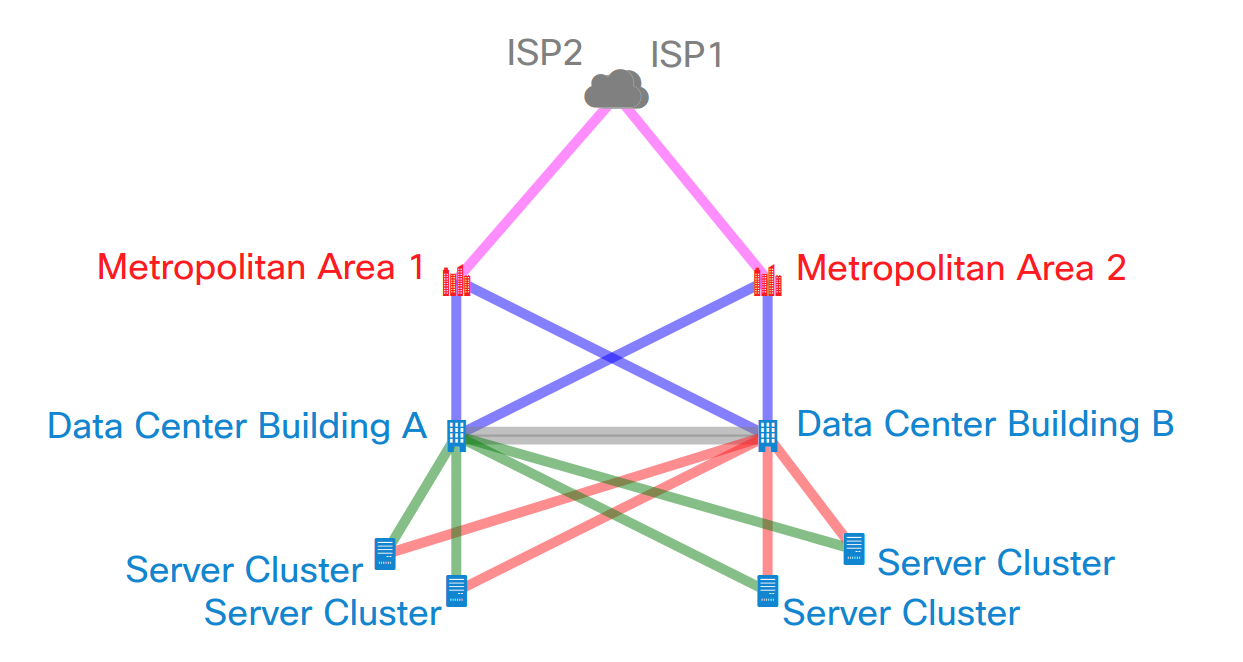
\includegraphics[scale=.2]{img/net_diag.png}
  \caption{General Topology of data center networks. The one to one metropolitan area to building relationships are shown for clarity only.}
  \label{fig:net_diag}
  \end{figure}


Large cloud data center operators have championed WAN systems for global up time and user experience optimizations \citep{sushant13} \citep{hong13}. Cloud data centers are a specific class of data centers that are comprised of custom information technology and building systems tuned for optimal total costs of ownership based on proprietary models at best or they optimized simple based on heuristics. These facilities house numerous services that can be controlled by network load balancers, with each data center limited by its physical infrastructure\textsc{\char13}s capacity. Given the applications described by Sushant and Hong, the network technology can shift loads on command, but doing so incurs additional costs for having hot spares. An effective hot spares strategy requires fully redundant replicas that, by design, would sit idle when other facilities are in operations. 

As noted by the enormous market value of data centers, businesses need robust models that can be used to assess the trade-offs between network flexibility and the physical infrastructure. The fungibility of locations enabled by the network technologies is also desirable from an application performance point of view as latency can be significantly reduced for specific markets and applications by reducing the round trip communication times with consumers. Given the popularity of the public clouds, the application of network aware energy model for data centers extends beyond just data center construction and plant operations.   

In the context of building energy modeling, WAN\textsc{\char13}s make the information technology workloads temporally (and geographically) unstable, rendering it elusively for building design professionals to reason about. As an example of temporal and geographical instability of data centers, Figure~\ref{fig:google_activity_dist} \citep{barroso18} shows the difference in utilization rates for two server clusters from their operational experience. The x-axis indicates the cumulative time ratio and the y-axis shows the utilization. The figure on the left shows that the peak utilization only happens for 40\% of the operational time. This is an area that building level energy simulations can help exploit. However, building energy simulation need to be aware of more then just energy. They must also be capable of quantifying the energy\textsc{\char13}s global warming potential in terms of carbon footprint.

  \begin{figure}
    \centering
    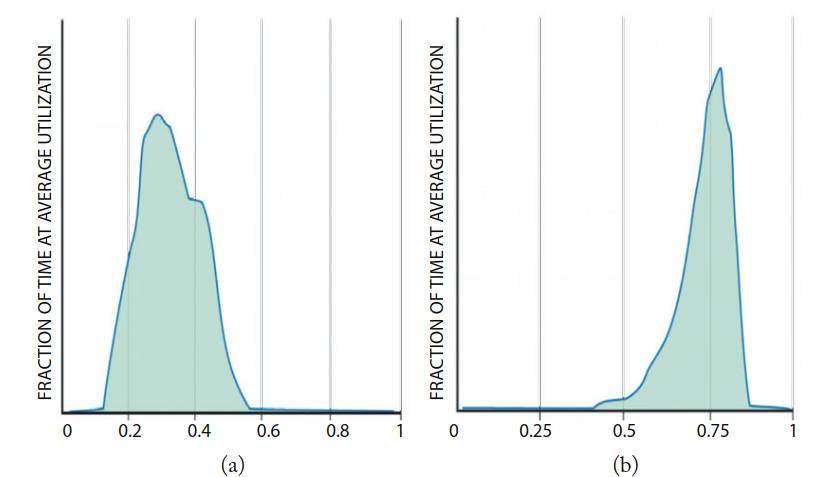
\includegraphics[scale=.2]{img/google_activity_dist.png}
    \caption{Average activity distribution of a sample of 2 clusters, each containing over 20,000 servers, over a period of 3 months. \citep{barroso18}}
    \label{fig:google_activity_dist}
    \end{figure}

Based on the literature reviews and references cited, there are no publicly available simulation frameworks that couple the dynamic data center workloads and the coincident carbon footprint associated with powering their load. The marginal cost of energy coupled building energy model described in this research is the first publicly available tool to allow owners, designers, and researchers to quantify the carbon footprint of data center operations accounting for granular supply and demand matching of power. Next, a literature review of past works concerning the carbon footprint of data-centers and digital services is presented in the Similar Works section.


%---------------------------------------------------------------------------------------
\section*{Similar Works}
%---------------------------------------------------------------------------------------
There are two notable past works that look at the energy footprint for distributed sets of data centers. First, Tripadi considers hardware capital costs alongside with energy acquisition costs to quantify the total costs of ownership in \citep{tripadi17}. Tripadi\textsc{\char13}s framework is dynamic in terms of workloads but it is not aware of the building energy dynamics. In the second work, Kiani and Ansari describe a geographical load balancing strategy that exploits green energy mix in the utility grid \citep{kiani17}. However, their load balancing scheme doesn\textsc{\char13}t provide insights into how the load balancer evaluates the building energy demands or how the greenness of the energy supply is obtained. 

Using a life cycle assessment framework, Whitehead demonstrates a comprehensive data center site level life cycle costs analysis in \citep{whitehead15}. All energy use in Whitehead’s models were deduced from annualized PUE values, precluding coincident energy source evaluations with their framework. Similarly the Green Grid’s data center life cycle assessment guideline is limited to PUE as their suggested basis for the operational energy proxy \citep{tgg12}.

Other’s have evaluated the costs of internet services \citep{koomey08} \citep{shehabi14}. Taylor and Koomey quantify the energy and greenhouse gas implications of online Advertising circa 2008. While Shehabi evaluates the energy and greenhouse gas implications of video stream circa 2014 \citep{shehabi14}. Together these works provide a taxonomy that can be followed to assess internet service costs in terms of energy use. 



%---------------------------------------------------------------------------------------
\section*{Methodology}
%---------------------------------------------------------------------------------------
In this section the marginal energy cost model\textsc{\char13}s coupling with the BEM is described. The resulting model maintains a strict partition between the two technical domains. The first part of the model simulates the hourly energy demands of a set of five data centers in EnergyPlus (EP) using the method demonstrated in \citep{kumar20}. These data centers are distributed across the globe as shown in Figure~\ref{fig:dc_locations}. Then in the second part, the data center demands are matched with the respective region\textsc{\char13}s utility power generation sources for the coincident hour to assess the marginal energy cost during that hour. These parts are described in the following subsections. 

\begin{figure}
  \centering
  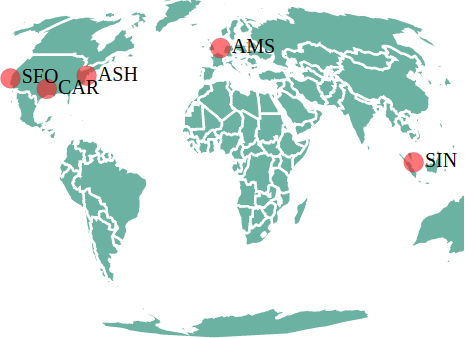
\includegraphics[scale=.40]{img/dc_locations.png}
  \caption{ Data center locations}
  \label{fig:dc_locations}
  \end{figure}


%---------------------------------------------------------------------------------------
\subsection*{Building Energy Model }
%---------------------------------------------------------------------------------------
For the first part, a sufficient building energy demand profile is simulated as in \citep{kumar20}.  The profile is obtained by using 50th quantile of the daily network traffic to each data center using Kumar’s method from \citep{kumar20b}.  However in lieu of using EP release 8.6, the simulation in this work uses EP release 8.9. The changes found EP 8.9 are listed in NREL’s GitHub \citep{nrel_git}. The programmatic changes from EPv8.9 resulted in three notable differences between original BEM and the model presented here.  The first change was motivated by original BEM's runtime errors when setting $2kW/m^2$ as the information technology (IT) equipment load density. This persistently led to thermal runaway conditions for the Singapore and San Francisco sites in EP release 8.9. In order to keep the building envelope form-factor and the construction materials the same, this simulation’s IT power load density is set to $1.0kW/m^2$.

The second change was made to exploit a new feature for modeling supply and return air compartmentalization in EP release 8.9. In these simulations, the data center model has air distribution flow control with approach temperatures specified. Flow control with approach temperature method calculates the temperature differences between the IT hardware boundaries and the air handling equipment.  This method is more representative of modern data-center operations and allows modeling ASHRAE 90.4 Standard’s requirement of hot-aisle / cold-aisle compartmentalization. The alternate method in EnergyPlus considers the entire data center room as a well-mixed environment, consistent with the modeling from \citep{kumar20}. While using the approach temperature method, the cooling temperature is changed for each time-step to 27 degrees Celsius from 25 degrees used in \citep{kumar20}. This 2-degree adjustment corresponds with the approach temperature between the air handling equipment discharge and the inlets of the ITE. 

As the third change, the load distribution specification in the IDF was revised from the SequentialLoad setting to UniformPLR. In the former, equipment is activated in the order listed in the IDF. With this specification each piece of equipment ramps sequentially from its idle state to full capacity, before subsequent equipment is enabled. In the latter load distribution specification, all equipment are loaded in parallel to each other. Another available setting for load distribution, the Optimal specification, was also tried for this field, but it crashed the simulations.

To validate that the proposed building energy model configurations are sufficient, with the above changes, each data-center is simulated with two models. In the first model, the economizer for the direct evaporative cooler (DEC) limits are relaxed while in the second model the default settings are maintained. The summary of the changes are indicated in Table~\ref{table:tab01}, while the comparison of total site energy between the two models for each set of the simulations is illustrated in Figure~\ref{fig:total_energy_comp}. A site\textsc{\char13}s pair simulations corresponds to the bars in the figure where the same data center is modeled with varying IDFs. In the figure the green bar indicates the total site energy of the model with economizer dry-bulb temperature limits relaxed. From the figure it is observed that the relaxed economizer leads to more energy use than the original values. While it maybe possible to fine optimal economizer settings, for this article it's concluded that the defaults settings from Kumar\textsc{\char13}s original work suffice. 

  
  \begin{table}[ht]
    \vspace{-10 pt}
    \caption{Relaxed economizer settings}
    \label{table:tab01}
    \centering
    \begin{tabular}{| c | c | c | }
      \hline
      \bf{IDF Object} & \bf{Variable} & \bf{Original/Econ} \\
      \hline
      DC-OA & Econ. Max db-C & 23 / 28 \\
      \hline
      DC DEC & Evap. Max db-C & 20 / 28 \\
      \hline
    \end{tabular}
    \vspace{-8 pt}   % Please use appropriate negative vspace to remove the space above/below the Table
    \end{table}

  \begin{figure}
    \centering
    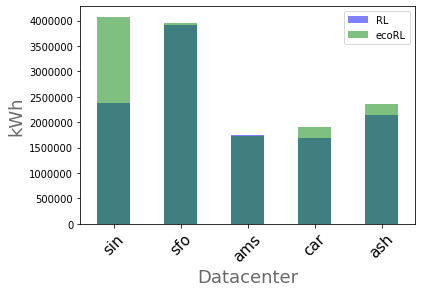
\includegraphics[scale=.45]{img/total_energy_comp.png}
    \caption{Comparison between relaxed economizer settings  vs. default IDF settings from \citep{kumar20} }
    \label{fig:total_energy_comp}
    \end{figure}

  The next subsection introduces the marginal costs of energy model,which will take the results from the original BEM.

%---------------------------------------------------------------------------------------
\subsection*{Regional Marginal Costs of Energy}
%---------------------------------------------------------------------------------------
The second module requires a time-series profile of the electrical grid’s power source attributions, where the time steps between the data center energy use profile match with the energy generation.  The corresponding  site and regional grid model pairs are indicated in Table~\ref{table:tab02}.For this model the energy generation regional grid profiles are obtained from Platt’s DOSCOE [5]. Singapore and Amsterdam data-centers grid profiles are constructed as described below.

\begin{table}[ht]
  \vspace{-10 pt}
  \caption{Data Center Site and Power Grid}
  \label{table:tab02}
  \centering
  \begin{tabular}{| c | c | c |  }
    \hline
    \bf{DC ID} & \bf{DC Location} & \bf{Regional Grid} \\
    \hline
    SFO & San Francisco, CA & California \\
    \hline
    CAR & Carrolton, Texas & ERCOT \\
    \hline
    ASH & Ashburn, VA & Midatlantic \\
    \hline
    AMS & Amsterdam & Netherlands \\
    \hline
    SIN & Singapore & Singapore \\
    \hline
  \end{tabular}
  \vspace{-10 pt}   % Please use appropriate negative vspace to remove the space above/below the Table
  \end{table}

  Each U.S region represented in the grid profiles is composed of hourly demands and corresponding production capacity of several power generation technologies. Hourly values for each region’s demand, solar, wind, coal, coal, coal with cryogenic capture, coal amine gas scrubbing, nuclear are defined. These grid regions are representative of three out of five of the data-center locations being simulated. 
  
  For Singapore, the International Energy Agency (IEA) provides a top down view of the annual energy production from various technologies. The IEA data shows that the renewable penetration in the energy supply for Singapore accounted for only 1.6\% of the total energy demand in 2016,the last year the data is available for \citep{IEA17}. Due to this negligible contribution from renewable sources and lack of hourly generation data, it is assumed that all demand is met by natural gas power generators, consistent with other sources \citep{eia20}.The demand profile for Singapore in 2016 is obtained from \citep{sin16}.

  For the Amsterdam data center, energy profile of Netherlands is used. The IEA indicates that in 2018, 12\% of Netherlands\textsc{\char13}s energy demands was met by renewable sources. This is a meaningful contribution from renewable, therefore a more granular generation profile is prudent.  To formulate the granular resolution of the generation, the IEA data is supplemented with data from the Open-Power-System-Data \citep{ospd19}. However, OPSD provides hourly data for the renewable sources only. The balance of the energy demands in the Netherlands is met by fossil fuel-based generators, namely 35\% by coal and 42\% by natural gas \citep{eia20b}. The DOSCOE grid profiles don’t have any corresponding field for bio-mass, so the bio-mass generation indicated in OPSD is lumped in with the fossil fuel generators. In the discussion section, some validation for this approach is presented. The Netherlands also produces nuclear energy, but only the annual production rates were obtained \citep{eia20b}. The annual nuclear production is distributed equally over the year and modeled as a constant (non-dispatchable) base load throughout the year.  

  The MEC coupled BEM algorithm is given below. In the algorithm two inputs are required. The first is DOSCOE[region], it is a two-dimensional array formatted as described in \citep{platt17}. It indicates hourly grid profiles of the power demand and power capacity of the available energy sources at the corresponding hour. The second inputs, traffic.language, is a one-dimensional vector indicating the network traffic to the respective site. Using the second input, for each language, (the proxy for an internet service) it’s traffic to the respective data center is checked. If there are traces of a language routed to a site, the algorithm performs the BEM simulation by invoking EnergyPlus. This resulting demands from EnergyPlus are then added to the region’s grid demand profile. If a language does not have any traffic to a particular site than, the data center site does not do any work and the BEM simulation is bypassed.  

  \begin{algorithm}
    \begin{small}
    \caption{MEC coupled BEM algorithm}
    \begin{algorithmic}
      \REQUIRE DOSCOE[region] \& traffic.language[site]
      \FOR{site and region in DC.site and DC.region}
        \IF{traffic.language[site].all $!= 0$: }
        \STATE $D_{DC} \gets BEM(site, traffic.language)$
        \STATE $DOSCOE[region].demand \pluseq demand[site]$
        \ENDIF
      \ENDFOR
      \STATE $CO_{2}$ {footprint}$\ =\ GridSim(region, rps)$
      \STATE{Where D = $DEMAND_{DC}$ }
    \end{algorithmic}
    \label{Service Profile}
  \end{small}
  \end{algorithm}

  The final step of algorithm quantifies the carbon footprint of the grid with the added data center loads by running DOSCOE’s Grid Simulator. In this step, the renewable portfolio standard (rps) argument specifies the percentage of renewable energy mix for the region.  

  In the next section the results from the methodology are discussed. 



%---------------------------------------------------------------------------------------
\section*{Discussion}
%---------------------------------------------------------------------------------------
The resulting values for source energy carbon footprint for each data center is summarized in Table~\ref{table:tab03} below. The energy model for the 491kW data center has been scaled by 1000 to represent the metro scale of data centers. The table further indicates the carbon footprint of each of the languages being served from the data centers. The values are indicative of the marginal amount of CO2 emitted by adding the data center demands to the grid. The units of the values are in Tons of $CO_2$ emitted.


\begin{table*}[ht]
  \vspace{-10 pt}
  \caption{Data Center Carbon Footprint}
  \label{table:tab03}
  \begin{small}
  \centering
  \begin{tabular}{|c c c c c c c c c| }
    \hline
    \bf{DC ID} & \bf{de} & \bf{en}    & \bf{es} & \bf{fr} & \bf{ja} & \bf{ru} & \bf{zh} & \bf{total}\\
    \hline
    SFO        & 0       & 1,301,549  & 0       & 0 & 0 & 0 & 0 & \bf{1,301,549}\\
    CAR        & 0       & 519,466    & 1,341,227  & 0 & 0 & 0 & 0 & \bf{1,860,693}\\
    ASH        & 0       & 563,085    & 1,109,162  & 661,919 & 0 & 0 & 0 & \bf{2,334,166}\\
    AMS       & 464,780      & 470,714   & 473,987  & 766,542 & 0 & 1,027,424 & 457,393 & \bf{3,660,840}\\
    SIN &  464,780      & 470,714   & 473,987  & 766,542 & 0 & 1,027,424 & 457,393 & \bf{3,660,840}\\
    \hline
    \bf{Sum} & \bf{464,780} & \bf{3,446,114}    & \bf{2,924,376} & \bf{2,042,611} & \bf{873,602} & \bf{1,888,019} & \bf{1,035,892} & \bf{12,675,394}\\
    \hline
  \end{tabular}
  \end{small}
  \vspace{-10 pt}   % Please use appropriate negative vspace to remove the space above/below the Table
  \end{table*}

From Table~ \ref{table:tab03} indicates the total marginal carbon footprint for each language by summing the language column. While the total marginal carbon footprint of each data center is obtained by summing the rows. The English pages have the most traffic globally and as expected English has the largest marginal carbon footprint due to its data-center operations. It is surprising however that the Netherlands data center has the highest total marginal carbon footprint among the data centers. A relatively lower marginal costs is expected due to the comparatively cooler ambient temperature in the Netherlands which would allow the data center systems to use economizers for more hours, but given that many languages are routed to the Amsterdam data center makes its absolute workload relatively is higher than other data centers. The EnergyPlus results support the lower building energy demands for the Netherlands site as shown in the stacked PUE histogram in \ref{fig:pue}. With the PUE values indicating the efficiency of the of the Netherlands site being more than average, the marginal carbon footprint can be attributed to the energy supply mix and higher network traffic from multiple languages. The aggregated the grid profile as described above for DOSCOE is heavily biased towards fossil fuels, therefore its carbon emissions are higher. This work used several secondary sources to construct the grid profile for the Netherlands and these sources may need to be validated more rigorously in the future.

As an implementation detail, the DOSCOE model proved to be quite sensitive to the data structure of the load profiles. For example any null value in the profile resulted in breaking the linear solver. Also, Solar and wind energy are required to be non-zero for at least one hour of the year. This requirement is a practical constraint, but in the profile developed for this work the values are arbitrarily set to a low value across all hours. Specifically, the defaults setting used in the work is 0.1 MW for each hour. 


%---------------------------------------------------------------------------------------
\section*{Conclusion}
%---------------------------------------------------------------------------------------
The network dependencies between physically dispersed data-center resources make system level building design decision a challenge to reason about. This research has presented a quantitative method to couple the network dependencies of data centers with their building energy and grid level marginal costs of energy. As shown for the Netherlands site, lower building level efficiencies, such has PUE does not equate to lower carbon footprint.  

As pointed out in the background section, there is a lack of bottoms up building design and carbon footprint models. The modular methodology of this research is a novel means of coupling abstracted service level metric, WAN traffic in this case, with physical based building energy simulation, EnergyPlus in this case. This integrated tool set can be used by data-center designers and operators to optimize their deployment across geographical bounds. Future work should consider controlling the network traffic based on building energy simulations to achieve global optimality in real time operational environments.  


\begin{figure}
  \centering
  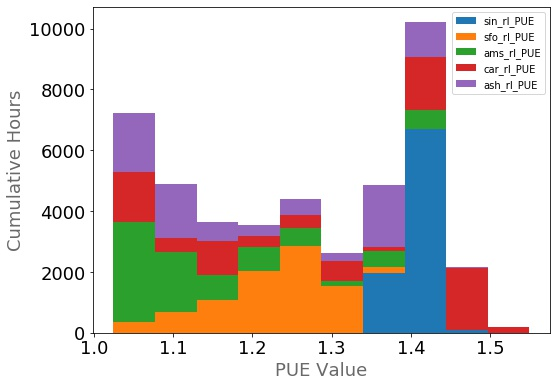
\includegraphics[scale=.40]{img/pue.jpg}
  \caption{Stacked histogram of PUE from all Data Centers.}
  \label{fig:pue}
  \end{figure}


%here starts the references
\newpage
\bibliographystyle{BS2020-Nordic.bst}
\bibliography{bibs}

\end{document}
